\documentclass{beamer}
\usepackage[english]{babel}
\usepackage[utf8]{inputenc}
\usepackage[T1]{fontenc}
\usepackage{lmodern}
\usepackage{hus-beamer}
\usepackage{ifthen}
%\usetikzlibrary{intersections}
\usepackage[bibstyle=authoryear, citestyle=authoryear, maxcitenames=2, maxbibnames=2, backend=bibtex]{biblatex}
%\usepackage[maxbibnames=2]{biblatex}
%citestyle=authoryear or numeric or ...
\addbibresource{export.bib}

%------ tikZ ------%
\usepackage{tikz}
\usetikzlibrary{tikzmark,overlay-beamer-styles,babel} 
\usetikzlibrary{positioning, arrows}
\usetikzlibrary{backgrounds}
    
\mode<presentation>{
	\usefonttheme{professionalfonts} % normal font for math formulas
	% insert section page with title only
	% before each section
	\AtBeginSection[]{
	\begin{frame}%[noframenumbering] % remove this if you do not want to number section page
	\vfill
	\centering
	\begin{beamercolorbox}[sep=8pt,center,shadow=true,rounded=true]{title}
	\usebeamerfont{title}\insertsectionhead\par%
	\end{beamercolorbox}
	\vfill
	\end{frame}
}
}
%%%%%%%%
%\AtBeginBibliography{\footnotesize} % Footnotesize for Bibliography entries

% \setbeamertemplate{bibliography item}{%
%   \ifboolexpr{ test {\ifentrytype{book}} or test {\ifentrytype{mvbook}}
%     or test {\ifentrytype{collection}} or test {\ifentrytype{mvcollection}}
%     or test {\ifentrytype{reference}} or test {\ifentrytype{mvreference}} }
%     {\setbeamertemplate{bibliography item}[book]}
%     {\ifentrytype{online}
%        {\setbeamertemplate{bibliography item}[online]}
%        {\setbeamertemplate{bibliography item}[article]}}%
%   \usebeamertemplate{bibliography item}}

% \defbibenvironment{bibliography}
%   {\list{}
%      {\settowidth{\labelwidth}{\usebeamertemplate{bibli<title>ography item}}%
%       \setlength{\leftmargin}{\labelwidth}%
%       \setlength{\labelsep}{\biblabelsep}%
%       \addtolength{\leftmargin}{\labelsep}%
%       \setlength{\itemsep}{\bibitemsep}%
%       \setlength{\parsep}{\bibparsep}}}
%   {\endlist}
%   {\item}


%\defbibheading{bibliography}[\refname]{}

%------------------%

\begin{document}
\title{Common network architectures}
%\subtitle{Week 4}
\author{COMP6252 (Deep Learning Technologies)}
\institute[ECS, University of Southampton]{ECS, University of Southampton} \date{28 April 2022}
 \date{}
\begin{frame}[plain,noframenumbering]
    \placelogofalse % No logo at the title page
    \titlepage
\end{frame}
    
\placelogotrue
\begin{frame}
	\frametitle{Learning outcomes}
\begin{enumerate}
	\item Be able to differentiate between object classification, single object localization and object detection

	\item Describe AlexNet/VGG/GoogLeNet/ResNet architectures
	\item Give a high-level description of fast RCNN
	\item Explain the functioning of the Inception module
	\item Explain the functioning of the residual module
\end{enumerate}
	

\end{frame}
\begin{frame}
    \frametitle{ImageNet dataset}
\begin{itemize}
    \item ImageNet is a massive dataset of images
    \item More than 14 million images in 20000 categories 
    \item Images are annotated with more than 1 million with bounding box
    \item Annual contest ImageNet Large Scale Visual Recognition Challenge (ILSVRC)
    \item ILSVRC classification uses  1000 distinct classes
    \item ILSVRC led to the development of architectures that are widely used in deep learning
\end{itemize}
    
\end{frame}
\begin{frame}
    \frametitle{ILSVRC}
    \begin{center}
        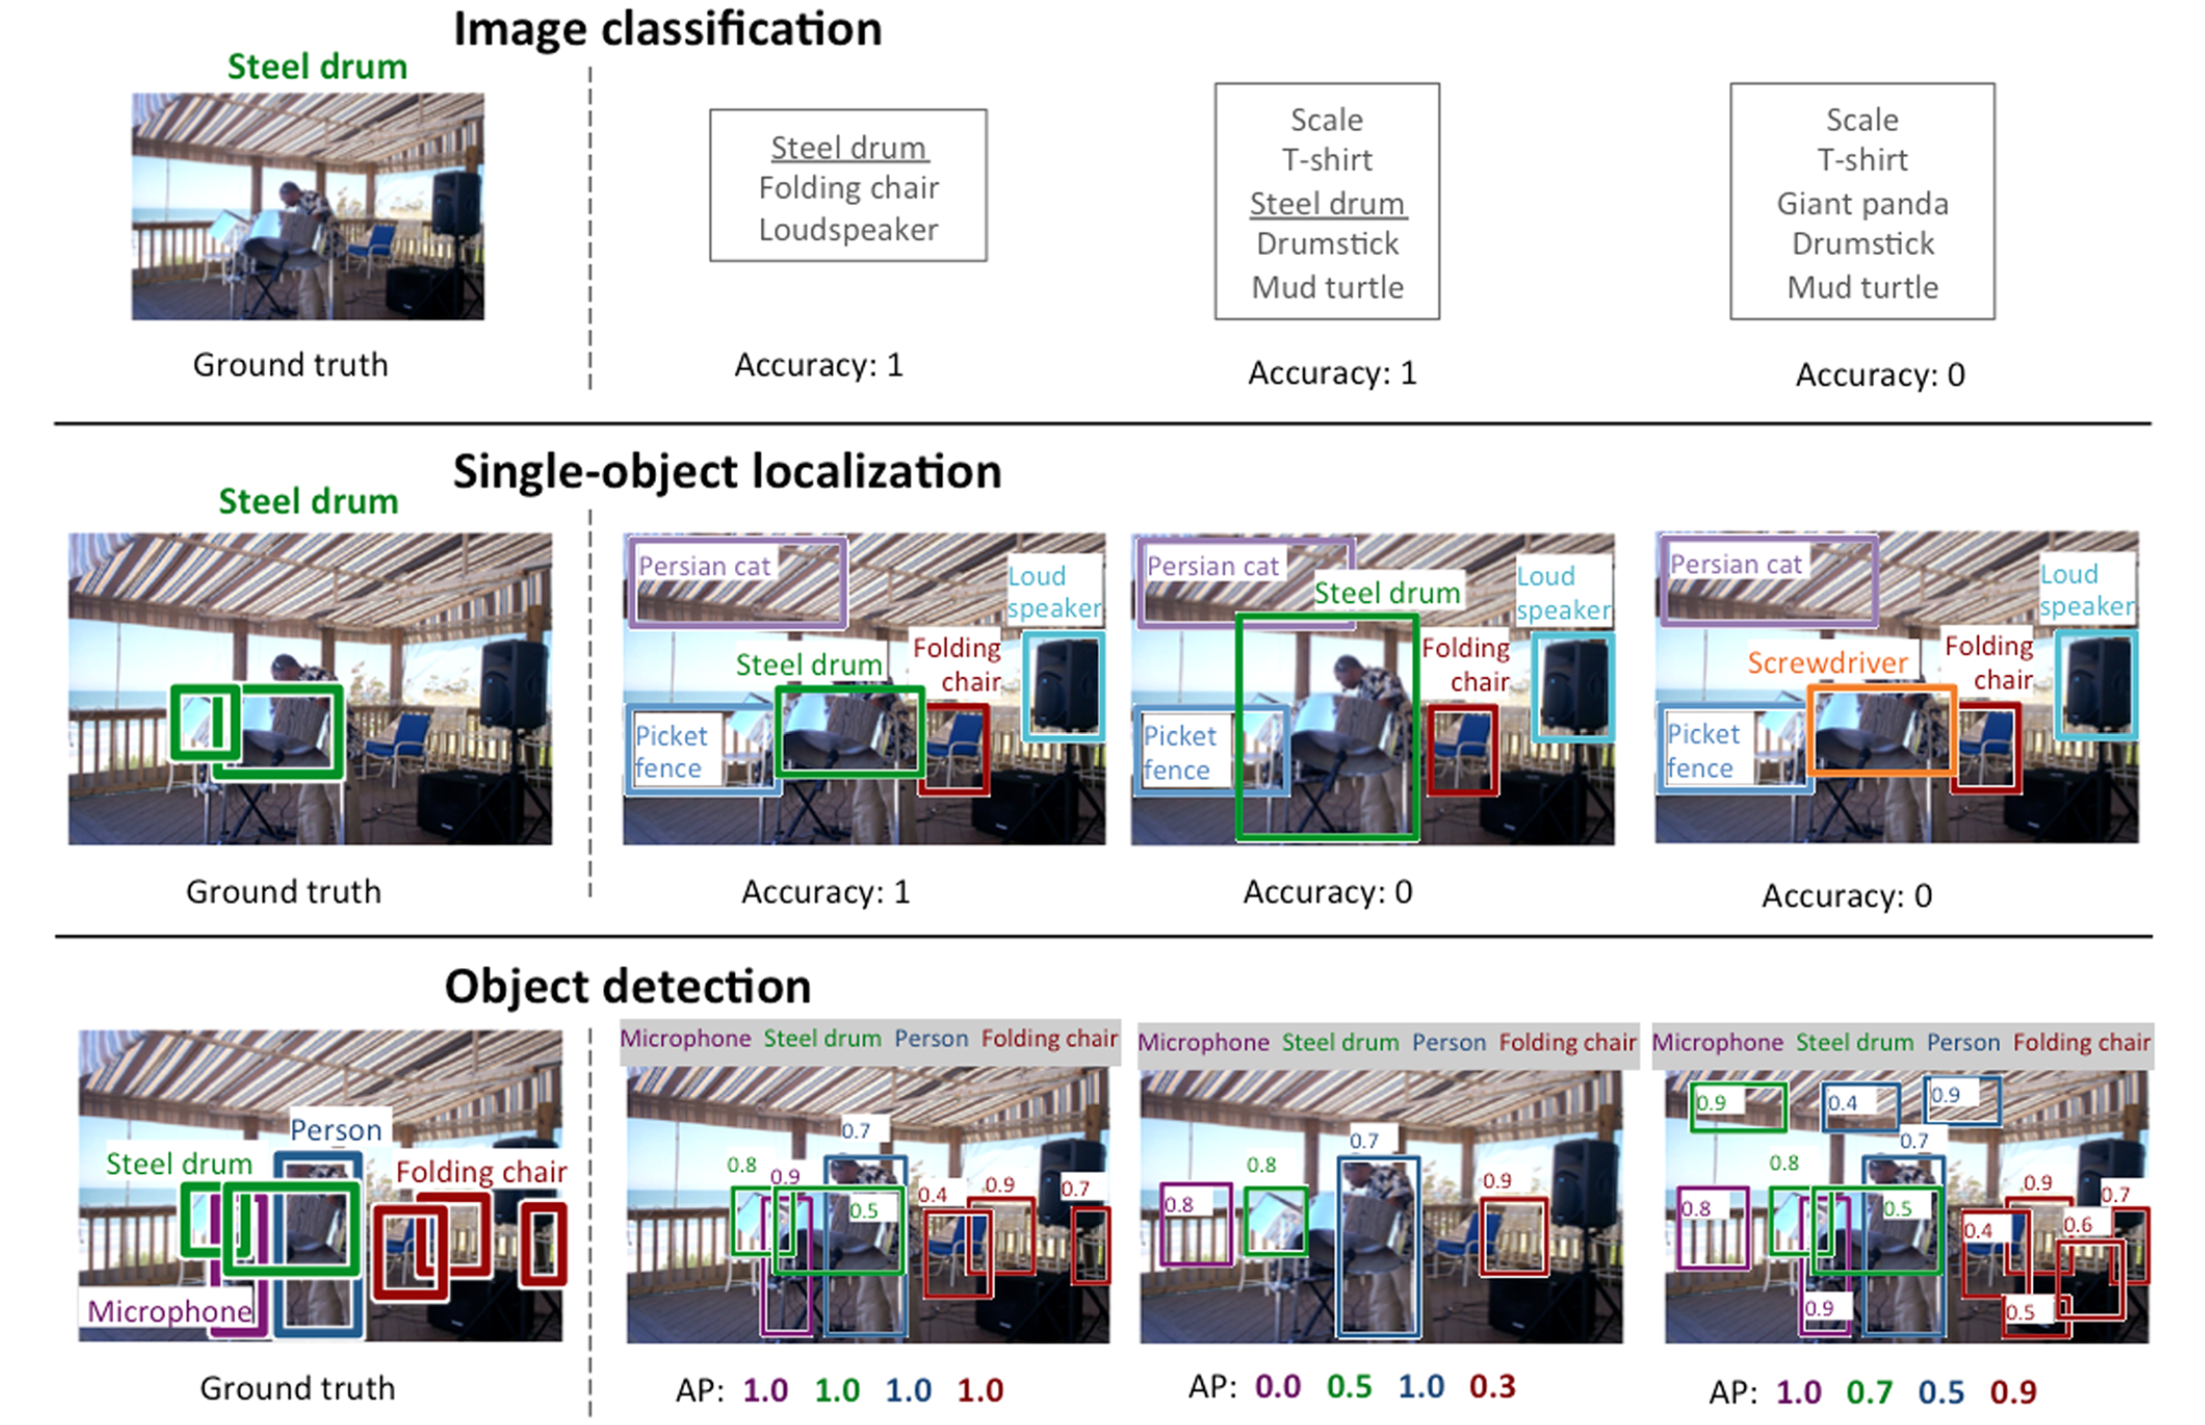
\includegraphics[width=\textwidth]{figs/ILSVRC.png}
    \end{center}
\end{frame}

\begin{frame}
    \frametitle{Top 5 errors}
    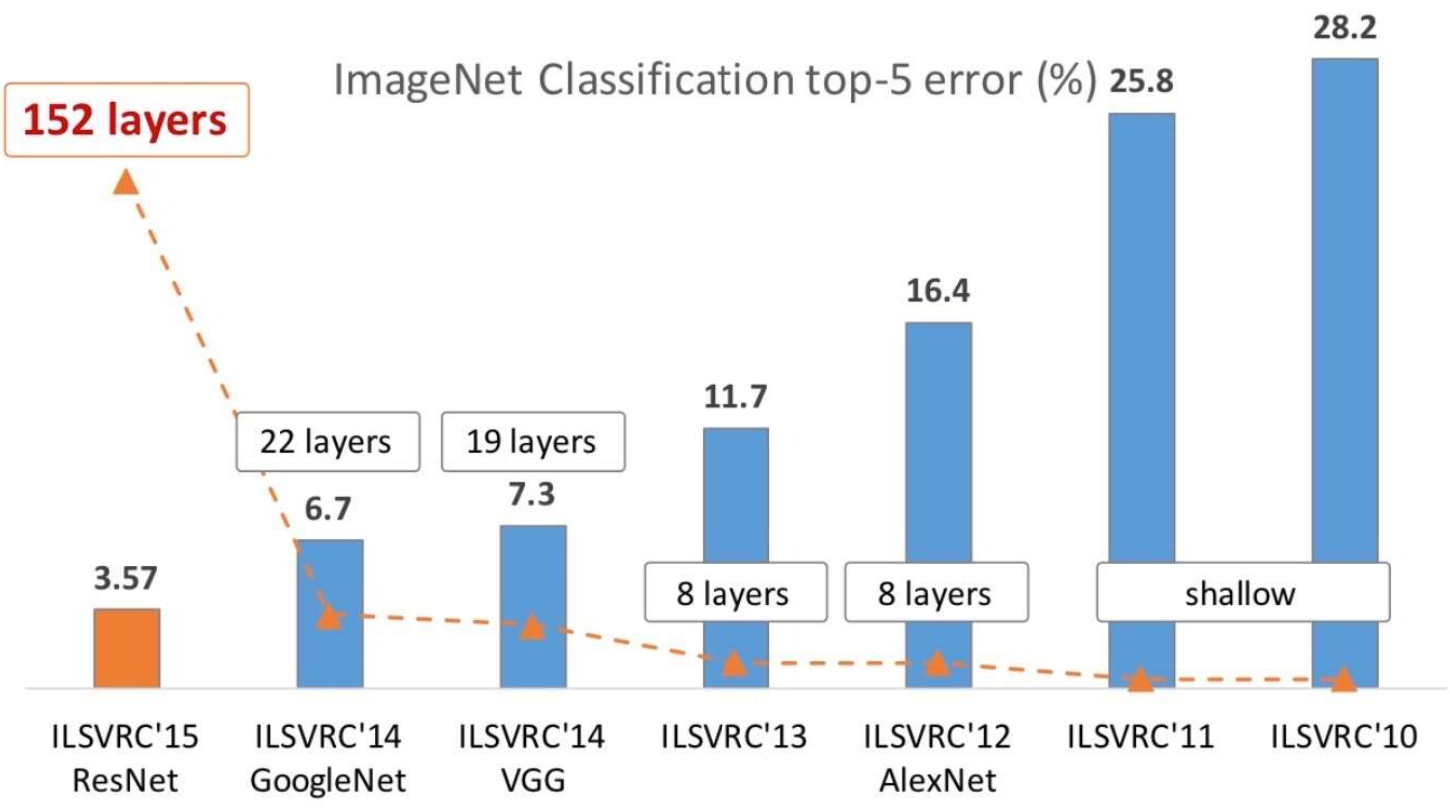
\includegraphics[width=\textwidth]{figs/top-5.png}
   \href{https://icml.cc/2016/tutorials/icml2016_tutorial_deep_residual_networks_kaiminghe.pdf}{\beamergotobutton{Image source}}
\end{frame}



\begin{frame}
    \frametitle{Alex net/VGG}
    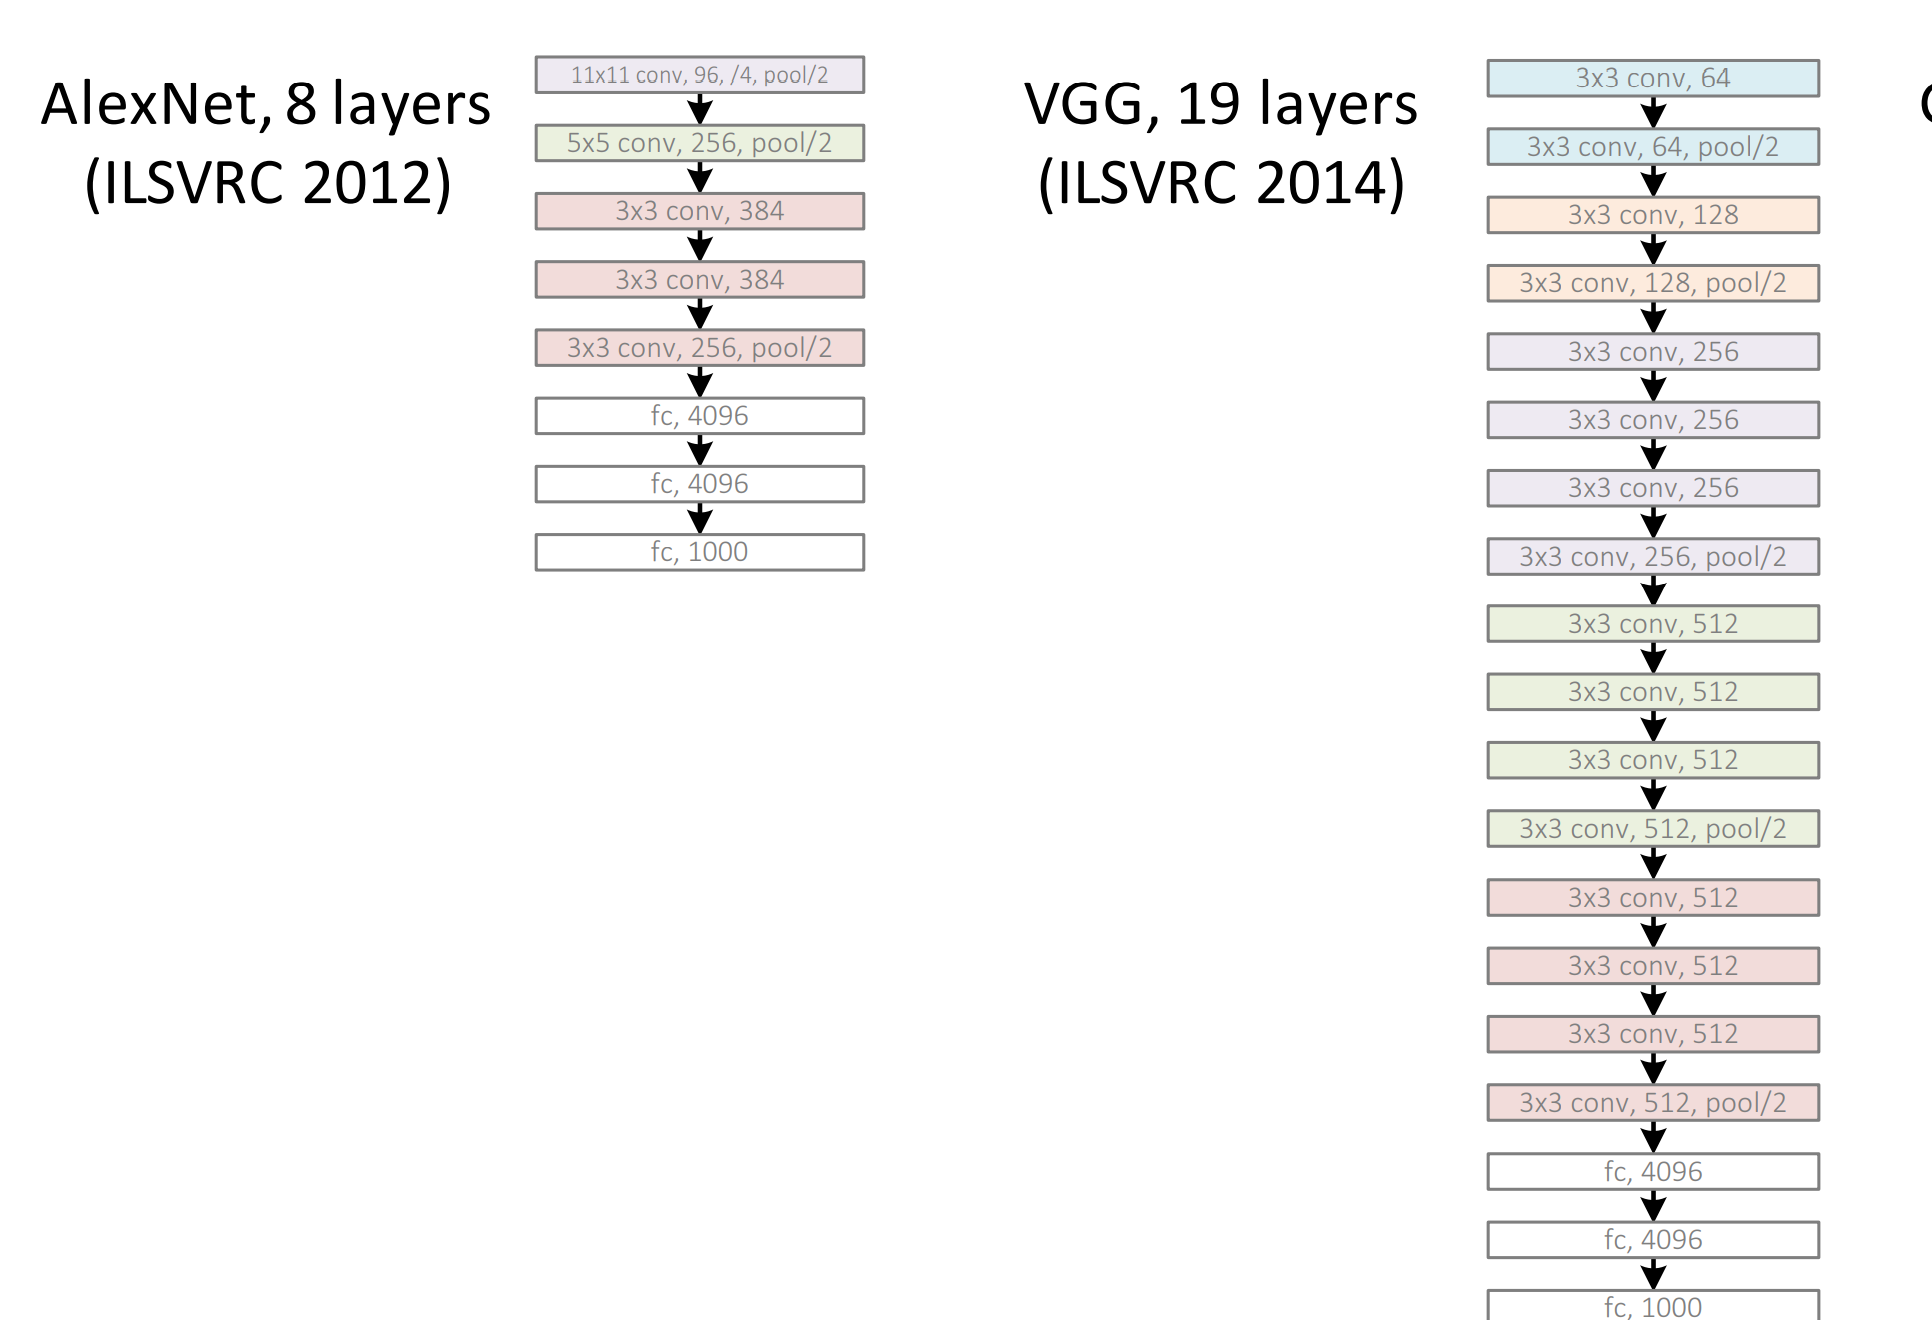
\includegraphics[width=\textwidth]{figs/alex-vgg.png}
   \href{https://icml.cc/2016/tutorials/icml2016_tutorial_deep_residual_networks_kaiminghe.pdf}{\beamergotobutton{Image source}}
\end{frame}

\begin{frame}
	\frametitle{Residual Networks}
\begin{itemize}
	\item Better results in image classification/recognition tasks when using deeper models 
	\item Can one keep adding layers  to get better results ?
	\item Initially deeper models faced the vanishing/exploding gradient problem
	\item That was solved using normalization techniques
	\item Another problem appeared when adding many layers: \textit{degradation of accuracy}
	\item Not caused by overfitting: \textbf{training} accuracy is degraded 
\end{itemize}
\end{frame}

\begin{frame}
    \frametitle{Training/test error}
\begin{center}
    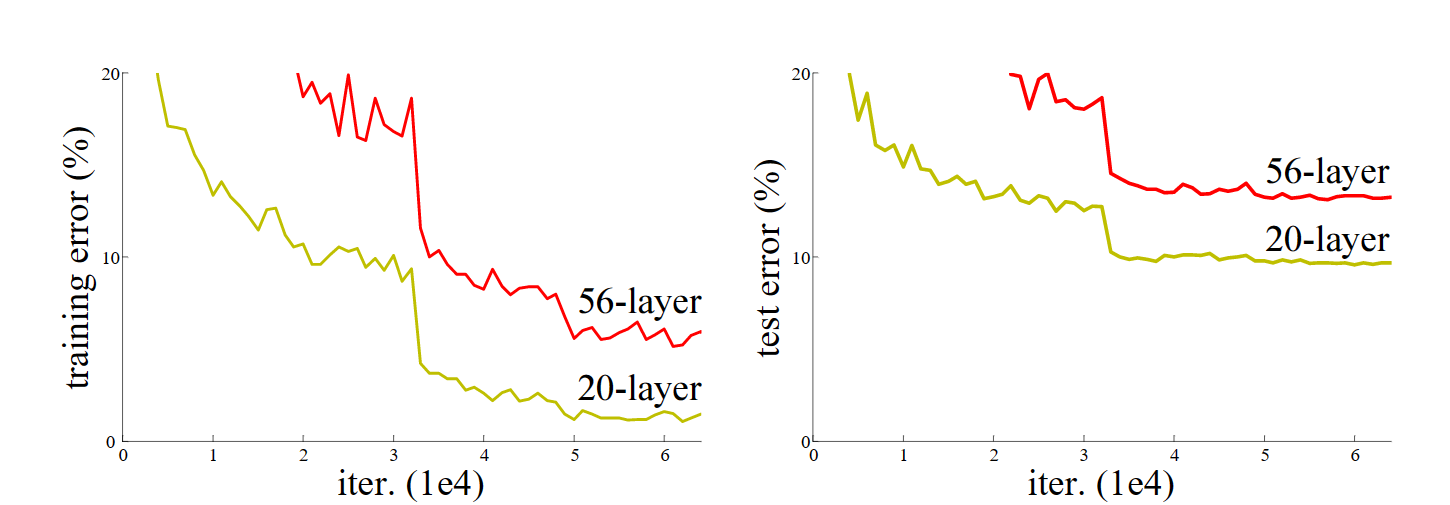
\includegraphics[width=\textwidth]{figs/deeper-error.png}
\end{center}

\end{frame}

\begin{frame}
	\frametitle{ResNet results}
\begin{itemize}
	\item First place in all categories of ILSVRC classification with 152 layers
	\item ILSVRC detection: 16\% better than 2nd
	\item ILSVRC localization: 27\% better than 2nd
\end{itemize}
	

\end{frame}



\begin{frame}
    \frametitle{Basic problem}
\begin{itemize}
    \item Consider a model $M$ of depth $d$
    \item Construct a deeper model $N$ which adds a single layer $I$ to $M$
    \item With $I(x)=x$ the identity map
    \item Basically the output of $M$ is used as input to $L$
    \item The above implies that $N$ should not give higher error than $M$
    \item It turns out it is hard to learn the identity map
\end{itemize}
\end{frame}
\begin{frame}
    \frametitle{Learning the identify map}

\begin{itemize}
    \item Consider a convolutional layer followed by a ReLU,$\sigma$
    \item Given an input $x$ we can write
    \begin{align*}
        y=\sigma(conv(x))
    \end{align*}
    \item Can one find a kernel such that
    \begin{align*}
        x=\sigma(conv(x))
    \end{align*}
     \item  Regardless of the output $conv(x)$, for $x<0$ the above equation cannot be satisfied 
\end{itemize}    

\end{frame}
\begin{frame}
    \frametitle{Basic idea}
\begin{itemize}
    \item What about learning the zero map?
    \item If the desired map to be learned is $\mathcal{H}(x)$
    \item Define $\mathcal{F}(x)=\mathcal{H}(x)-x$
    \item Now if a component learns $\mathcal{F}(x)$
    \item All we have to do is add $x$ to the output
    \item This is done by adding a \textbf{skip} connection or a \textbf{shortcut}
\end{itemize}

\end{frame}
\begin{frame}
    \frametitle{Residual module}

    \begin{center}
        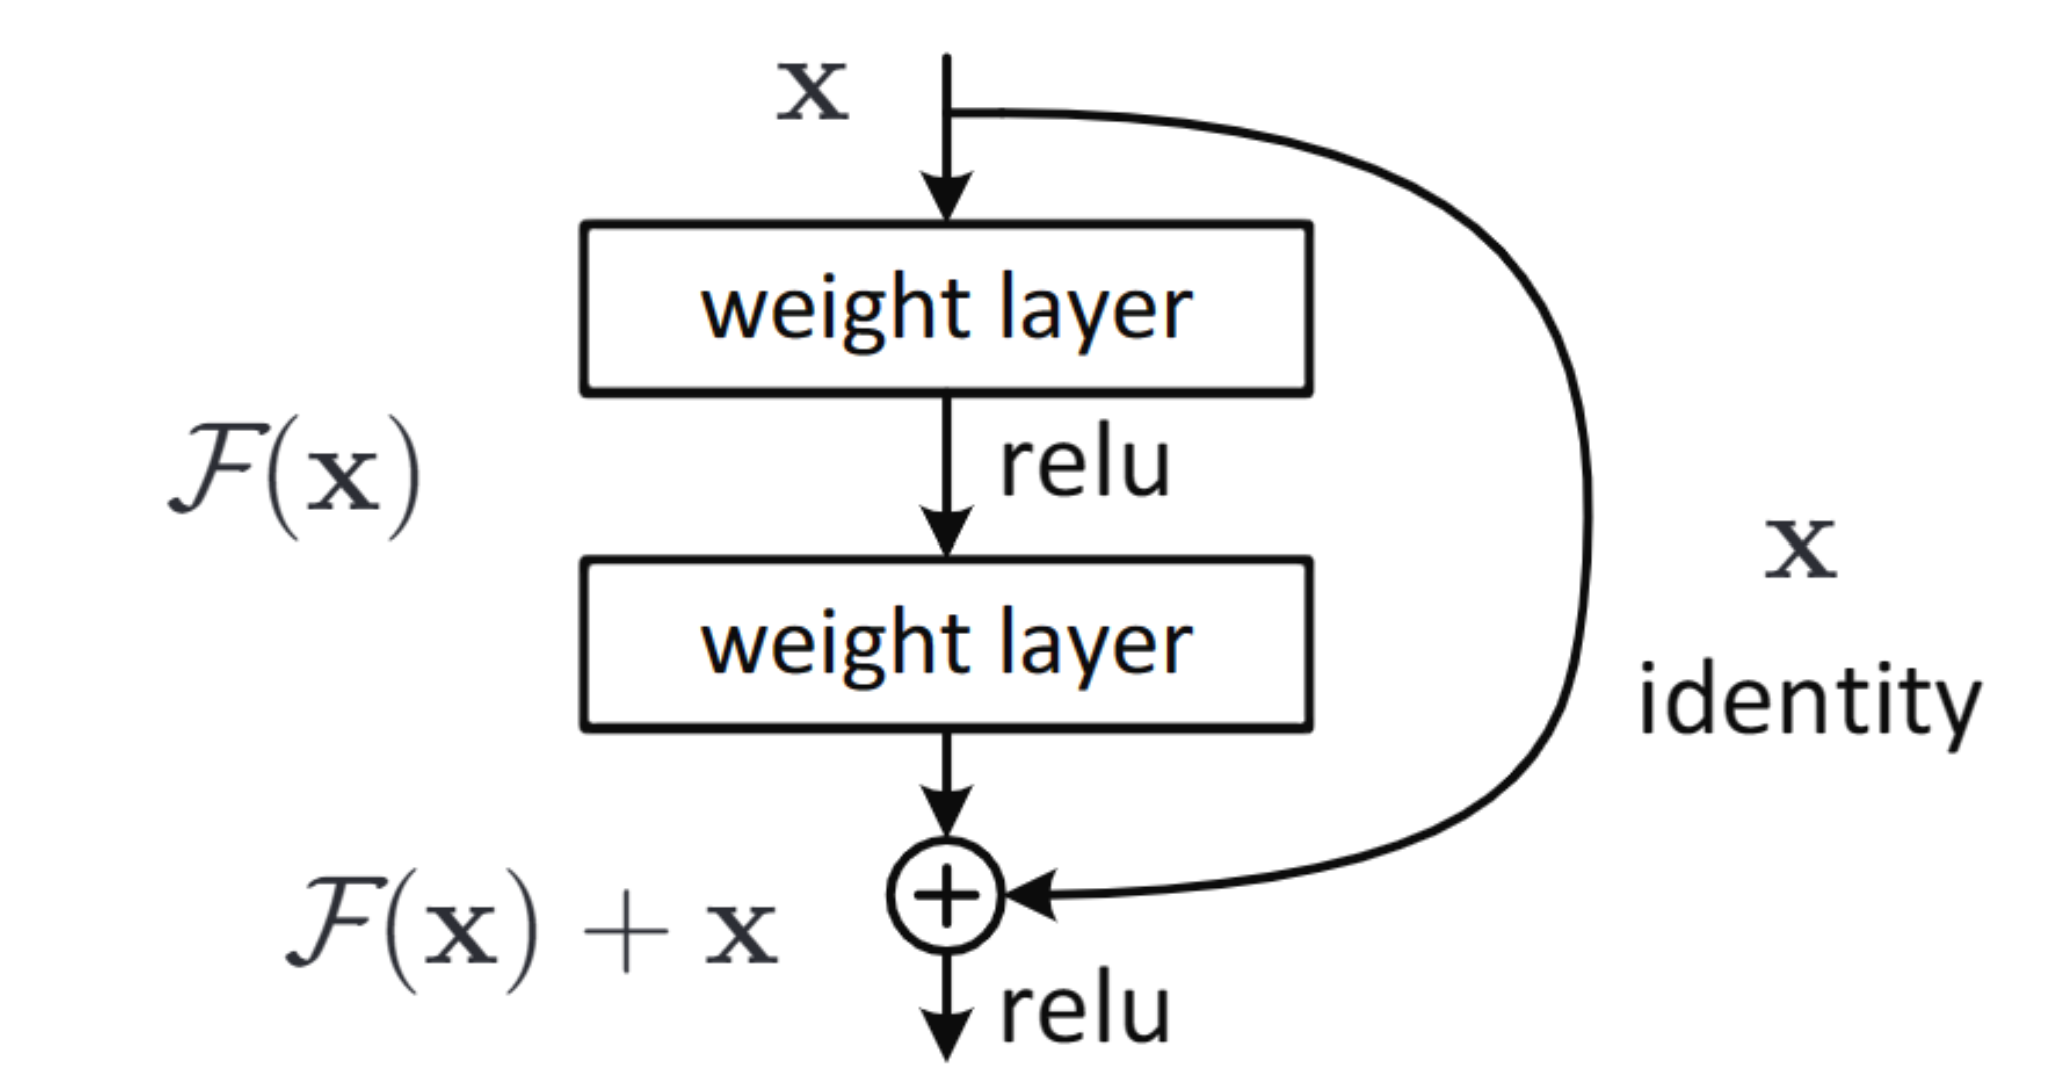
\includegraphics[width=\textwidth]{figs/residual-block.png}
    \end{center}
\end{frame}
\begin{frame}
    \frametitle{Resnet 34}

    \begin{center}
        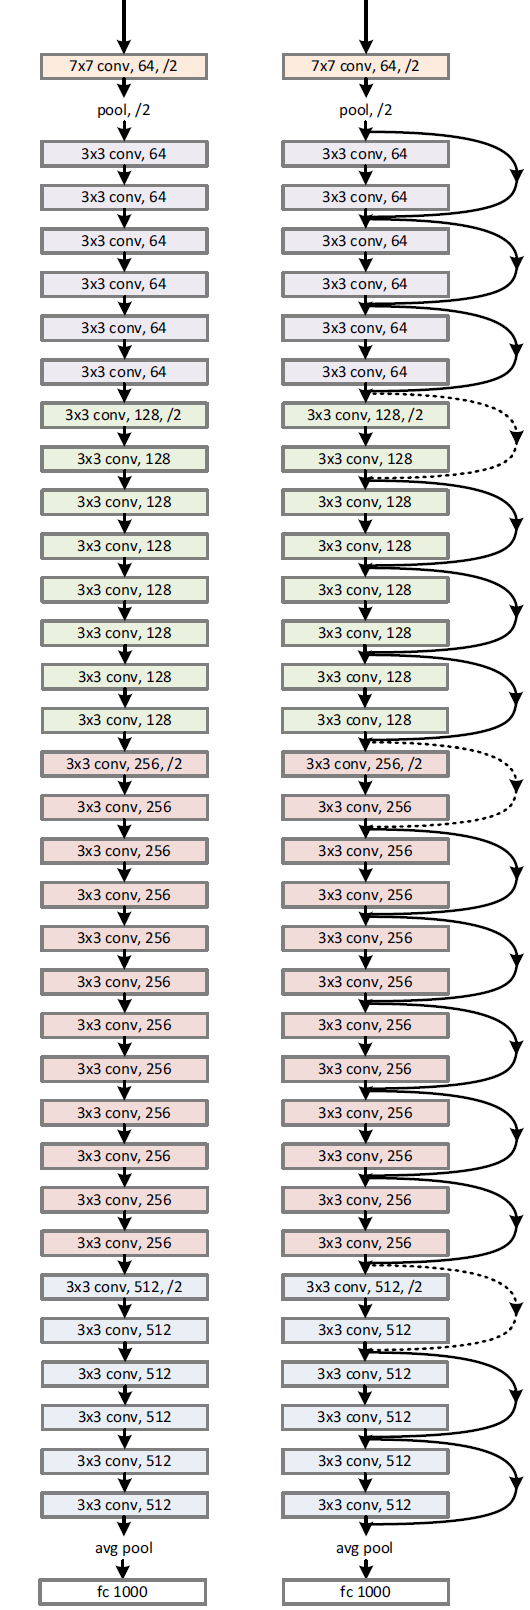
\includegraphics[width=0.22\textwidth]{figs/resnet34.png}
    \end{center}

\end{frame}
\begin{frame}
    \frametitle{Inception (GoogLeNet)}
	\begin{columns}
		
\begin{column}{0.5\textwidth}

    \begin{itemize}
        \item Stack Inception modules on top of each other
        \item Network within a network
    \end{itemize}

    \begin{figure}
        \tikzmarknode{module}{
            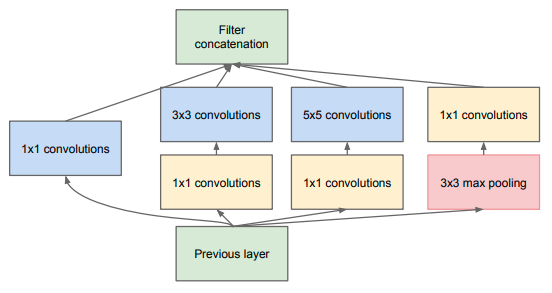
\includegraphics[width=1.1\textwidth]{figs/inception.png}
        }
    \end{figure}
		
\end{column}
\begin{column}{0.5\textwidth}
	\vspace{-1.5cm}
	\begin{figure}
        \tikzmarknode{net}{
            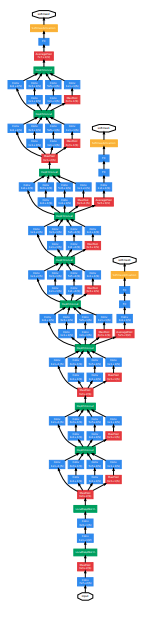
\includegraphics[width=0.4\textwidth]{figs/googlenet.png}
        }
    \end{figure}
\end{column}
\end{columns}
\begin{tikzpicture}[overlay,remember picture]
	%\draw [draw=red] (7.5,2.98) rectangle (9.6,4);
	\node (rect) at (8.5,2.73) [draw=red,thick,minimum width=2cm,minimum height=0.8cm] {};
	\draw[-latex,color=red] (rect.west) to (module.east);
	\end{tikzpicture}
\end{frame}

\begin{frame}
	\frametitle{Auxiliary classifiers}
\begin{itemize}
	\item there are 9 inception modules
	\item 3a,3b,4a,4b,4c,4d,4e,5a,5b
	\item Auxiliary classifiers with softmax are attached to 4a and 4d
	\item Their output are added to the total loss (with 0.3 weight)
	\item Their role is to minimize vanishing gradient effect by injecting additional gradient at lower layers
	\item They also act as regularizers to minimize overfitting
	\item During inference their output is discarded 
\end{itemize}
	

\end{frame}


\begin{frame}
	\frametitle{Naive Inception}
\begin{columns}
	\begin{column}{0.5\textwidth}

	\begin{figure}
        \tikzmarknode{naive}{
            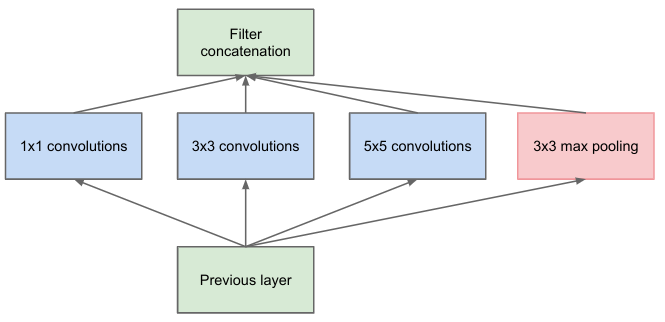
\includegraphics[width=1.1\textwidth]{figs/naive_inception.png}
        }
    \end{figure}
\end{column}
\begin{column}{0.5\textwidth}
	\begin{itemize}
		\item Filters applied in parallel
		\item The results are concatenated over the channels
		\item Geometric dimensions of convolutions and maxpooling are the same 
		\item MaxPooling with 3x3 kernel stride=1 and padding=1 to preserve the dimensions
		\item All convolutions are padded so no change in height/width
	\end{itemize}
\end{column}
\end{columns}

\end{frame}

\begin{frame}
	\frametitle{Inception vs Naive Inception}
\begin{columns}
	\begin{column}{0.5\textwidth}
		\begin{figure}
			\tikzmarknode{naive}{
				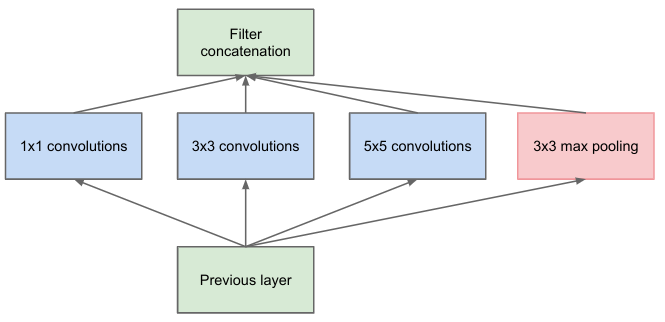
\includegraphics[width=1.\textwidth]{figs/naive_inception.png}
			}
		\end{figure}
	\end{column}
	\begin{column}{0.5\textwidth}
		\begin{figure}
			\tikzmarknode{naive}{
				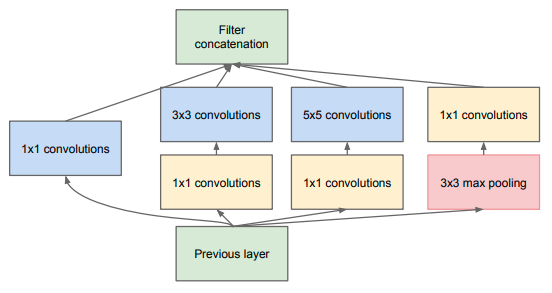
\includegraphics[width=1.\textwidth]{figs/inception.png}
			}
		\end{figure}
	\end{column}
\end{columns}
\end{frame}

% \begin{frame}
% 	\frametitle{Role of 1x1 convolution}
% \begin{itemize}
% 	\item preserves spatial dimensions but reduces depth
% \end{itemize}
	

% \end{frame}


% \begin{frame}
% 	\frametitle{Naive Inception}
% \begin{columns}
% 	\begin{column}{0.5\textwidth}

	
% 	\begin{figure}
%         \tikzmarknode{naive}{
%             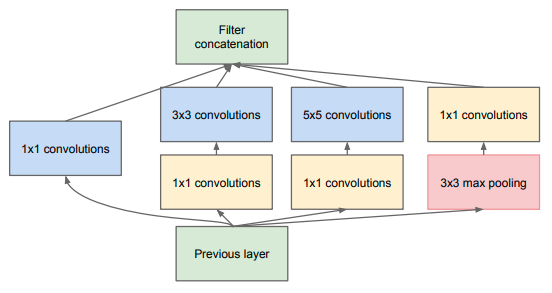
\includegraphics[width=1.3\textwidth]{figs/inception.png}
%         }
%     \end{figure}
% \end{column}
% \hfill
% \begin{column}{0.4\textwidth}
% 	Multiplication operations
% \tiny{
% 	\begin{itemize}
% 		\item 1x1: 192x28x28x1x1x64=9633792
% 		\item 3x3: 192x28x28x3x3x128=173408256
% 		\item 5x5: 192x28x28x5x5x32=120422400
% 		\item Total$\approx $ 303M ops
% 	\end{itemize}
% 		}
	
% \end{column}
% \end{columns}

% \end{frame}

\begin{frame}
	\frametitle{Inception module}
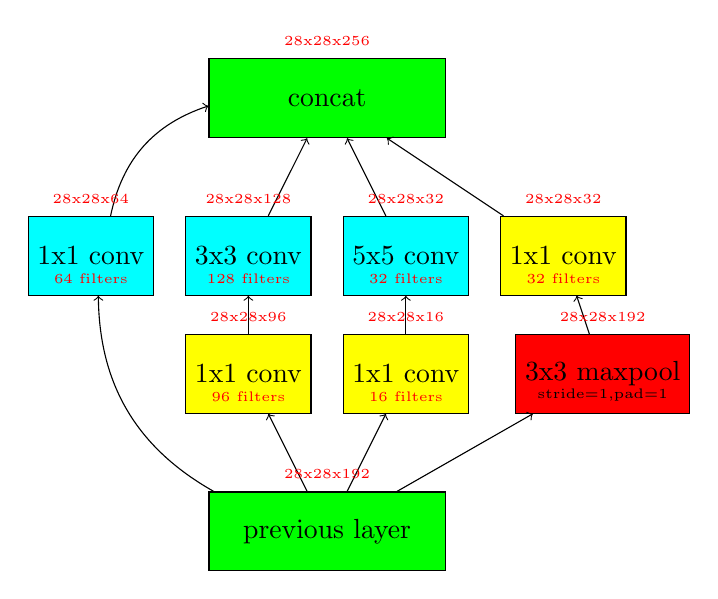
\begin{tikzpicture}
	\node (1x1a) at (0,2) [fill={rgb,1:green,1;blue,1},minimum width=1.5cm,minimum height=1cm,draw] {1x1 conv};
	\node (3x3) at (2,2) [fill={rgb,1:green,1;blue,1},minimum width=1.5cm,minimum height=1cm,draw] {3x3 conv};
	\node (5x5) at (4,2) [fill={rgb,1:green,1;blue,1},minimum width=1.5cm,minimum height=1cm,draw] {5x5 conv};
	\node (1x1b) at (6,2) [fill={rgb,1:red,1;green,1},minimum width=1.5cm,minimum height=1cm,draw] {1x1 conv};
	\node (1x1c) at (4,0.5) [fill={rgb,1:red,1;green,1},minimum width=1.5cm,minimum height=1cm,draw] {1x1 conv};
	\node (1x1d) at (2,0.5) [fill={rgb,1:red,1;green,1},minimum width=1.5cm,minimum height=1cm,draw] {1x1 conv};
	\node (maxpool) at (6.5,0.5) [fill={rgb,1:red,1},minimum width=1.5cm,minimum height=1cm,draw] {3x3 maxpool};

	\node (prev) at (3,-1.5) [fill={green},minimum width=3cm,minimum height=1cm,draw] {previous layer};
	\node (next) at (3,4) [fill={green},minimum width=3cm,minimum height=1cm,draw] {concat};
	\path[->] (prev) edge [bend left=3em] (1x1a);
	\path[->] (prev) edge  (1x1c);
	\path[->] (prev) edge  (1x1d);
	\path[->] (prev) edge  (maxpool);
	\path[->] (1x1a) edge  [bend left=3em] (next);
	\path[->] (3x3) edge  (next);
	\path[->] (5x5) edge  (next);
	\path[->] (1x1b) edge  (next);
	\path[->] (1x1d) edge  (3x3);
	\path[->] (1x1c) edge  (5x5);
	\path[->] (maxpool) edge  (1x1b);
	%shapes 
	\node[text=red] (maxpoollabel) [node distance=1pt,above=of maxpool]{\tiny 28x28x192};
	\node[text=red] (1x1alabel) [node distance=1pt,above=of 1x1a]{\tiny 28x28x64};
	\node[text=red] (1x1dlabel) [node distance=1pt,above=of 1x1d]{\tiny 28x28x96};
	\node[text=red] (5x5label) [node distance=1pt,above=of 5x5]{\tiny 28x28x32};
	\node[text=red] (3x3label) [node distance=1pt,above=of 3x3]{\tiny 28x28x128};
	
\node[text=red] (output) [node distance=1pt ,above= of next]{\tiny 28x28x256};
	
	\node[text=red] (1x1clabel) [node distance=1pt,above=of 1x1c]{\tiny 28x28x16};
	\node[text=red] (1x1dfilters) [node distance=1pt,above=of 1x1d.south]{\tiny 96 filters};
	\node[text=red] (1x1cfilters) [node distance=1pt,above=of 1x1c.south]{\tiny 16 filters};

	\node[text=red] (1x1afilters) [node distance=1pt,above=of 1x1a.south]{\tiny 64 filters};
	\node[text=red] (3x3filters) [node distance=1pt,above=of 3x3.south]{\tiny 128 filters};
	\node[text=red] (5x5filters) [node distance=1pt,above=of 5x5.south]{\tiny 32 filters};


	\node[text=black] (maxpoolfilter) [node distance=1pt,above=of maxpool.south]{\tiny stride=1,pad=1};
	
	\node[text=red] (1x1bfilters) [node distance=1pt,above=of 1x1b.south]{\tiny 32 filters};
	\node[text=red] (1x1label) [node distance=1pt,above=of 1x1b]{\tiny 28x28x32};
	\node[text=red] (prevlabel) [node distance=1pt,above=of prev]{\tiny 28x28x192};
\end{tikzpicture}
	

\end{frame}



\begin{frame}
	\frametitle{Naive Inception module}
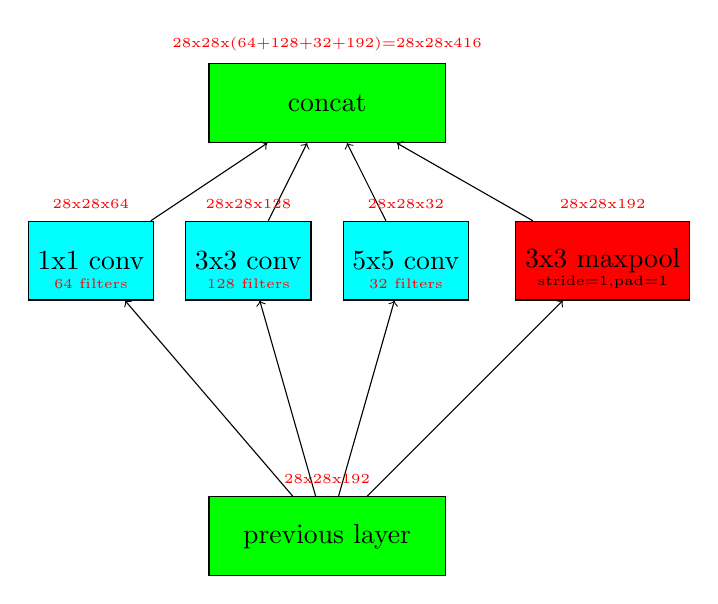
\begin{tikzpicture}
	\node (1x1a) at (0,2) [fill={rgb,1:green,1;blue,1},minimum width=1.5cm,minimum height=1cm,draw] {1x1 conv};
	\node (3x3) at (2,2) [fill={rgb,1:green,1;blue,1},minimum width=1.5cm,minimum height=1cm,draw] {3x3 conv};
	\node (5x5) at (4,2) [fill={rgb,1:green,1;blue,1},minimum width=1.5cm,minimum height=1cm,draw] {5x5 conv};
	
	\node (maxpool) at (6.5,2) [fill={rgb,1:red,1},minimum width=1.5cm,minimum height=1cm,draw] {3x3 maxpool};

	\node (prev) at (3,-1.5) [fill={green},minimum width=3cm,minimum height=1cm,draw] {previous layer};
	\node (next) at (3,4) [fill={green},minimum width=3cm,minimum height=1cm,draw] {concat};
	%\path[->] (prev) edge [bend left=3em] (1x1a);
	\path[->] (prev) edge (1x1a);
	
	\path[->] (prev) edge  (maxpool);
	\path[->] (prev) edge  (3x3);
	\path[->] (prev) edge  (5x5);
	\path[->] (maxpool) edge  (next);
	\path[->] (1x1a) edge  (next);
	%\path[->] (1x1a) edge  [bend left=3em] (next);
	\path[->] (3x3) edge  (next);
	\path[->] (5x5) edge  (next);
	
	%shapes 
	\node[text=red] (maxpoollabel) [node distance=1pt,above=of maxpool]{\tiny 28x28x192};
	\node[text=red] (1x1alabel) [node distance=1pt,above=of 1x1a]{\tiny 28x28x64};
	
	\node[text=red] (5x5label) [node distance=1pt,above=of 5x5]{\tiny 28x28x32};
	\node[text=red] (3x3label) [node distance=1pt,above=of 3x3]{\tiny 28x28x128};
	
\node[text=red] (output) [node distance=1pt ,above= of next]{\tiny 28x28x(64+128+32+192)=28x28x416};
	
	
	\node[text=red] (1x1afilters) [node distance=1pt,above=of 1x1a.south]{\tiny 64 filters};
	\node[text=red] (3x3filters) [node distance=1pt,above=of 3x3.south]{\tiny 128 filters};
	\node[text=red] (5x5filters) [node distance=1pt,above=of 5x5.south]{\tiny 32 filters};


	\node[text=black] (maxpoolfilter) [node distance=1pt,above=of maxpool.south]{\tiny stride=1,pad=1};
	
	\node[text=red] (prevlabel) [node distance=1pt,above=of prev]{\tiny 28x28x192};
\end{tikzpicture}
\end{frame}

\begin{frame}
	\frametitle{Multiplication operations}

	\begin{itemize}
		\item To estimate the complexity of the (naive) inception module we count the multiplication operations
		\item input $H\times W\times C$ with $F$ filters of size $K\times K$
		\item since stride=1 and padding=same then filter is "strided" $H\times W$ times
		\item Each time it performs $K\times K \times C$ operations for a total of $H\times W\times C\times K\times K$ ops 
		\item There are $F$ filters so the total is $H\times W\times C\times K\times K\times F$
	\end{itemize}

\end{frame}
\begin{frame}
	\frametitle{Naive vs reduced inception }
	\begin{itemize}
		\item Naive inception
		\begin{itemize}
			\item 1x1 conv: $28\times 28\times 192\times 1 \times 1\times 64\approx 9.6M$
			\item 3x3 conv: $28\times 28\times 192\times 3 \times 3\times 128\approx 173.4M$
			\item 5x5 conv $28\times 28\times 192\times 5 \times 5\times 32\approx 120	.4M$
			\item Total $303M$ operations
		\end{itemize}
		\item Reduced inception
	
\begin{itemize}
	\item 1x1 conv $28\times 28\times 192\times 1\times 1 \times(64+96+16+32)\approx 31 M$
	\item 3x3 conv $28\times 28\times 192\times 3\times 3\times 128\approx 87M$
	\item 5x5 $28\times 28\times 16\times 5\times 5\times 32\approx 10M$

	\item Total $128M$ operations
\end{itemize}
\end{itemize}

\end{frame}
\begin{frame}
	\frametitle{Object detection}
	\begin{center}
        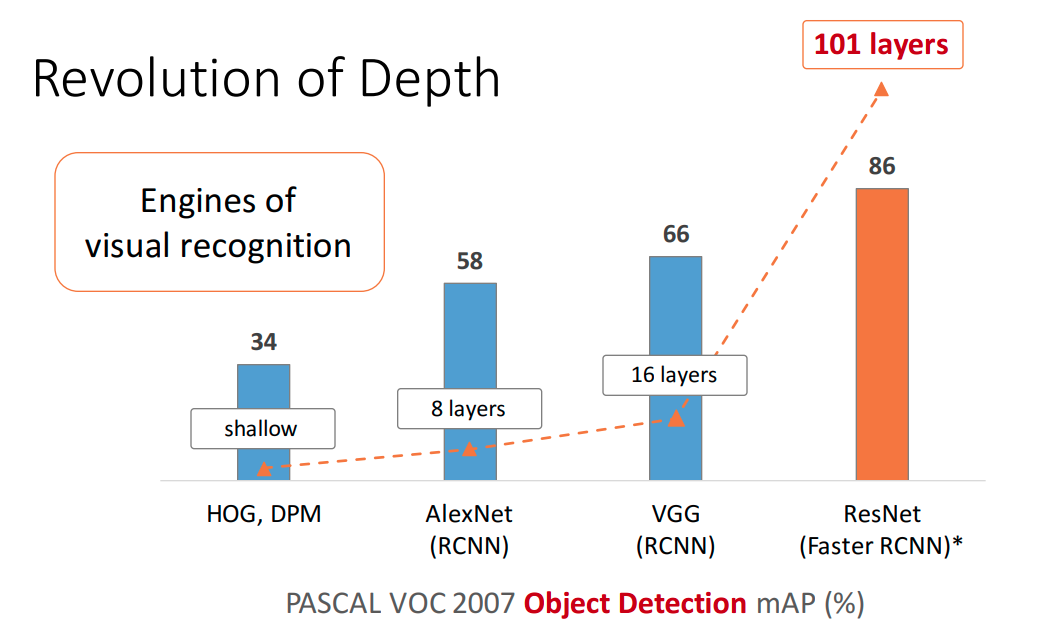
\includegraphics[width=\textwidth]{figs/object-detect.png}
    \end{center}
	

\end{frame}
\begin{frame}
	\frametitle{Object detection}
\begin{itemize}
	\item Image localization: bounding box
	\begin{itemize}
		\item Uses intersection over union (IOU) threshold
		\item Usually threshold 0.5
	\end{itemize}
	
	\item Object classification: cat/dog/etc...
	\item Most common measure is mean average precision (mAP)
	\begin{itemize}
		\item mean average precision(mAP): AP=area under the precision/recall curve
		\item precision/recall computed using both correct label and bounding box
	\end{itemize}
\end{itemize}
\end{frame}
\begin{frame}
	\frametitle{Intersection over union}
\begin{center}
	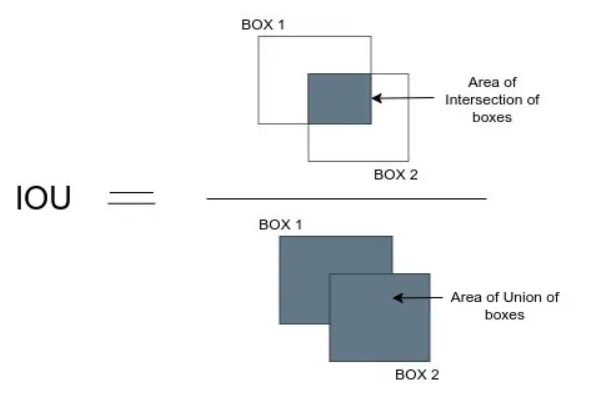
\includegraphics[width=\textwidth]{figs/iou.png}
\end{center}
\end{frame}
\begin{frame}
	\frametitle{Precision and Recall}
	\begin{center}
		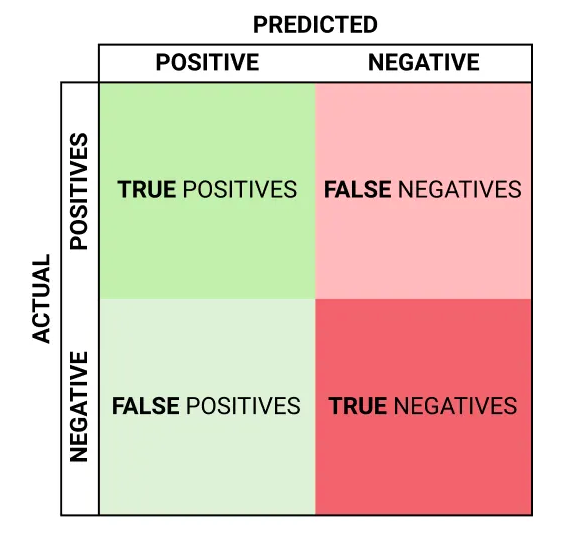
\includegraphics[width=0.5\textwidth]{figs/confusion-mat.png}
		\href{https://towardsdatascience.com/precision-and-recall-88a3776c8007}{\beamergotobutton{Image source}}
	\end{center}
\begin{itemize}
	\item Precision $\frac{TP}{TP+FP}$
	\item Recall $\frac{TP}{TP+FN}$
\end{itemize}
\end{frame}

\begin{frame}
	\frametitle{Fast RCNN}
\begin{center}
	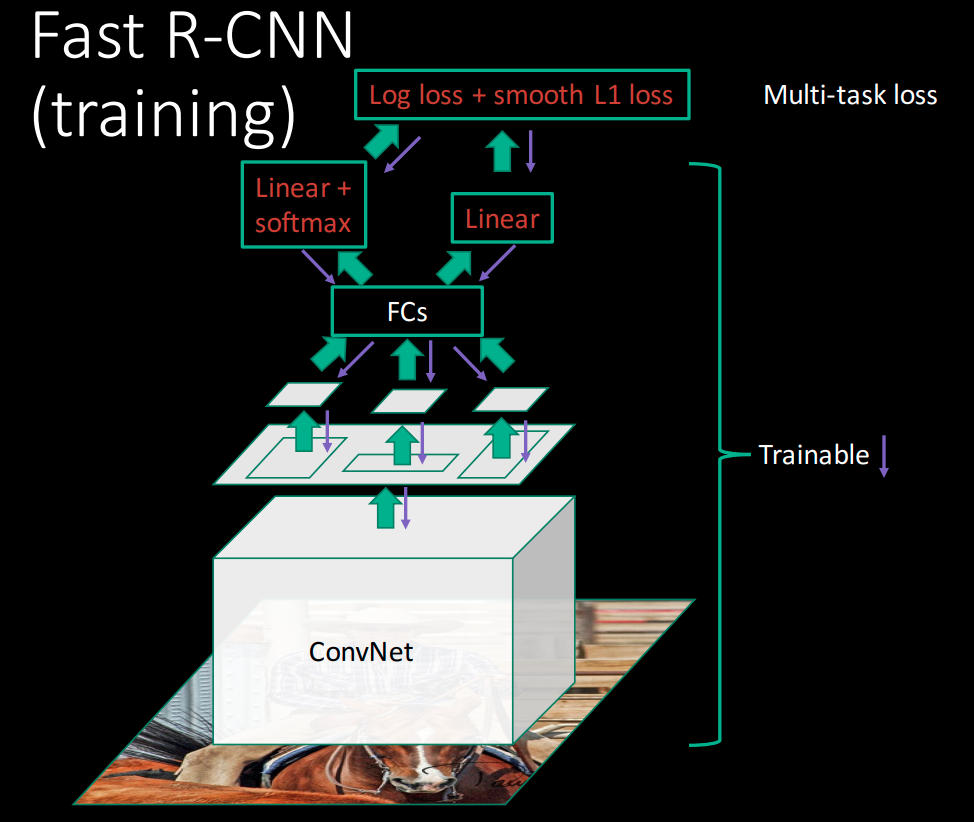
\includegraphics[width=0.7\textwidth]{figs/fast-rcnn.png}
\end{center}
	

\end{frame}



\begin{frame}
    \frametitle{References}
    % \begin{itemize}
    %     \item \cite{srivastava14}\cite{ioffe15}
    % \end{itemize}
	\nocite{*}    

\printbibliography

\end{frame}
\end{document}